\documentclass[a4paper]{jpconf}
\usepackage{graphicx}
\begin{document}
\title{Speech segregation based-on binaural cue: interaural time difference (itd) and interaural level difference (ild)}

\author{Mifta Nur Farid, Dhany Arifianto}

\address{Dept. of Engineering Physics, Faculty of Industrial Technology, Institut Teknologi Sepuluh Nopember, Kampus ITS Sukolilo, Surabaya 60111, Indonesia}

\ead{miftanurfarid@gmail.com}

\begin{abstract}
A person who is suffering from hearing loss can be helped by using hearing aids and the most optimal performance of hearing aids are binaural hearing aids because it has similarities to human auditory system. In a conversation at a cocktail party, a person can focus on a single conversation even though the background sound and other people conversation is quite loud. This phenomenon is known as the cocktail party effect. In an early study, has been explained that binaural hearing have an important contribution to the cocktail party effect. So in this study, will be performed separation on the input binaural sound with 2 microphone sensors of two sound sources based on both the binaural cue, interaural time difference (ITD) and interaural level difference (ILD) using binary mask. To estimate value of ITD, is used cross-correlation method which the value of ITD represented as time delay of peak shifting at time-frequency unit. Binary mask is estimated based on pattern of ITD and ILD to relative strength of target that computed statistically using probability density estimation. Results of sound source separation performing well with the value of speech intelligibility using the percent correct word by 86\% and 3 dB by SNR.
\end{abstract}


\section{Introduction}
Hearing impairment has been an area of ​​research in recent years. Despite the common cause is due to age, excessive noise exposure also reduce hearing ability (hearing loss)\cite{kates2008}. A person who is suffering from hearing loss can be helped by using hearing aids. Kind of hearing aids that provide the most optimal performance if hearing loss in both ears are binaural hearing aids \cite{marin2012} because it has similarities to the human auditory system.


The auditory system can separate many sound source simultaneously. For example, in a conversation at a cocktail party, a person can focus on single conversation even though the background sound and other people conversation is quite loud. This phenomenon is known as the cocktail party effect\cite{cherry1957}. The term "cocktail party processing" created in an initial study on the cocktail party effect, this study illustrates that binaural hearing provides an important contribution in auditory analysis that allows us to isolate and localize the sound source\cite{hawley2004}.


In binaural hearing, if the position of a sound source is not in the median plane hence one ear will be overshadowed by the head while the other ear is fully open to the sound source. The result is a difference in the sound pressure level that is heard in both ears, is called Interaural Level Difference (ILD) and the differences in travel time of the sound source to the ears is called Interaural Time Difference (ITD). According to Roman\cite{roman2002}, changes in the value ITD and ILD, statistically, has the effect to the changes of Relative Strength (RS). So binary mask can be estimated from the value of the RS that obtained by the changes ​​of ITD and ILD in time-frequency domain. So in this study, will be performed separation on the binaural sound input with 2 microphone sensors of two sound sources based on both the binaural cue, interaural time difference (ITD) and interaural level difference (ILD) using binary mask.


To estimate value of ITD, is used cross-correlation method which the value of ITD represented as time delay of peak shifting at time-frequency unit. Then the binary mask is estimated based on pattern of ITD and ILD to relative strength of target that computed statistically using probability density estimation.

The rest of paper is organized as follows. Section 2 describes the process of data training. Section 3 describes the segregation processing. Section 4 present evaluation of segregation results. Section 5 is result and discussion while the last Section 6 is conclusion.

\section{Data Training Process}
\subsection{Binaural Hearing}
In this process, spatial information will be given to a target signal and a masker signal by convoluting them with HRTF (head-related transfer function). The HRTF database that used is "HRTF Measurement of Kemar Dummy-Head Microphone" from MIT Media Lab Perceptual Computing. The HRTF database contained head-related impulse response of both ear in anechoic room with distance to sound source is 1.4 m. The location of sound source is azimuth $0^o$ for a target and $5^o$, $10^o$, $20^o$, and $30^o$ for a masker.

\subsection{Auditory Periphery}
The results of binaural hearing processing only simulate the sound transmission on the outer ear, so it is necessary to simulate the middle and inner ear using auditory periphery processing. Auditory periphery contained 3 stages. The first stage is gammatone-filter, which is the target and masker signal filtered using $4^{th}$order gammatone-filter 

\begin{equation}\label{pers:gammatone}
g(t) ~=~ at^{3}e^{-2\pi bt}\cos(2 \pi ft + \phi)
\end{equation}

with 128 center frequencies distributed in scale ERB 80 Hz to 5000 Hz\cite{roman2002}.

\begin{equation}\label{pers:erb}
ERB(f) ~=~ 24.7 \left( \frac{4.37 f}{1000} + 1\right)
\end{equation}

The second stage is middle ear gain that provides gain to simulate the effects of middle-ear function based on equal-loudness of BS3383, Normal Equal-Loudness Level. And the last is the hair cells that model the activity of the auditory-nerve that represented by firing-probability in inner ear\cite{meddis1986}.

\subsection{Binaural Cue Extraction}
Interaural time difference (ITD) is estimated as the time delay corresponding to the position of the maximum value of the cross-correlation results of $C(i, j, \tau)$ between the pair HRTF on $i$-frequency channels, $j$-time frame, and $\tau$-lag \cite{jeffress1948}.
\begin{equation}\label{pers:itd}
C(i, j, \tau) ~=~ \frac{\sum_{k=0}^{K-1}(l_i(j-k)-\bar{l_i})(r_i(j-k-\tau)-\bar{r_i})}{\sqrt{\sum_{k=0}^{K-1}(l_i(j-k)-\bar{l_i})^2}\sqrt{\sum_{k=0}^{K-1}(r_i(j-k)-\bar{r_i})^2}}
\end{equation}

where $l_i$, $r_i$ is firing-probabilty of left ear and right ear at $i$-frequency channel, and $\bar{l_i}$, $\bar{r_i}$ is the average value of firing-probabilty at $K$-integration window.

Interaural level difference (ILD) is estimated as

\begin{equation}\label{pers:ild}
ILD_i = 20log_{10}\frac{\sum_i l_i^2(t)}{\sum_i r_i^2(t)}
\end{equation}

where $l_i$, $r_i$ is firing-probabilty of left ear and right ear at $i$-frequency channel.

\subsection{Relative Strength Estimation}
Relative strength is energy ratio between target to mixed signal. Relative strength is estimated as

\begin{equation}
RS_i = \frac{\sum_i s_i^2(t)}{\left(\sum_i s_i^2(t) + \sum_i n_i^2(t)\right)}
\end{equation}

where $s_i$ is the target signal and $n_i$ is the masker signal at $i$-frequency channel.

\subsection{Probability Density Estimation}
At this stage, the analysis of patterns between both ITD and ILD to the relative strength of a target signal to mixed signal in the time-frequency unit. Pattern analysis conducted by estimating the probability density that represent the statistical relationship between those values (ITD, ILD and relative strength). Estimation of probability density performed at the relative strength of two types, the value of probability density when a target signal is more dominant than a masker signal ($RS > 0.5$) and a masker signal are more dominant or equal than a target signal ($RS \leq 0.5$) in time-frequency domain.


\begin{figure}[h]
    \centering
    \includegraphics[width=5.5in]{pict/pde.eps}
    \caption{\label{pict:pde}Probability Density Estimation for ITD and ILD to (a) relative strength ($RS \ge 0.5$) and (b) ($RS \leq 0.5$) of target and masker at $0^o$ and $30^o$ with SIR 10 dB and center frequency 500 Hz}
\end{figure} 


The results of probability density estimation (PDE) for both types of relative strength of a single target and masker at $0^o$ and $30^o$ with SIR 10 dB and center frequency 500~Hz shown in figure \ref{pict:pde}. In figure \ref{pict:pde} (a), the highest peak occurs in the value of ITD = 0 ms, which means the relative strength values is greater than 0.5 more distributed on these, whereas in figure \ref{pict:pde} (b) highest peak occurs at ITD = 0.8 ms, which means relative strength value is less than or equal to 0.5 more distributed in that ITD. Black line in figure \ref{pict:pde} (a) and (b), which represents the distribution of the value of ILD at target, is shorter than the ILD in the masker (red line). The results corresponding to reduction of relative strength value if the position of the sound source away from the median plane. From here it can be concluded, to estimate the binary mask that requires a value relative strength can be estimated with only the known value of the ITD and ILD alone on the mixtured signal.

\section{Segregation Process}
\subsection{Azimuth Estimation}
Azimuth of the target signal and masks can be estimated from summing the results of cross-correlation between the mixtured signal on the left ear and right ear in the time domain on all center frequency of 80 Hz to 5000 Hz. The peak value of the sum of cross correlation in ITD function can be represented as azimuth in figure \ref{pict:azimuth}. In this figure, the first peak is at a lag of $0~ms$ is defined as a azimuth of target signal and a second peak at $0.21~ms$ as azimuth of masker signal. Both of these values as parameters of decision to take probability density estimation database of the results of the training data.

\begin{figure}[h]
    \centering
    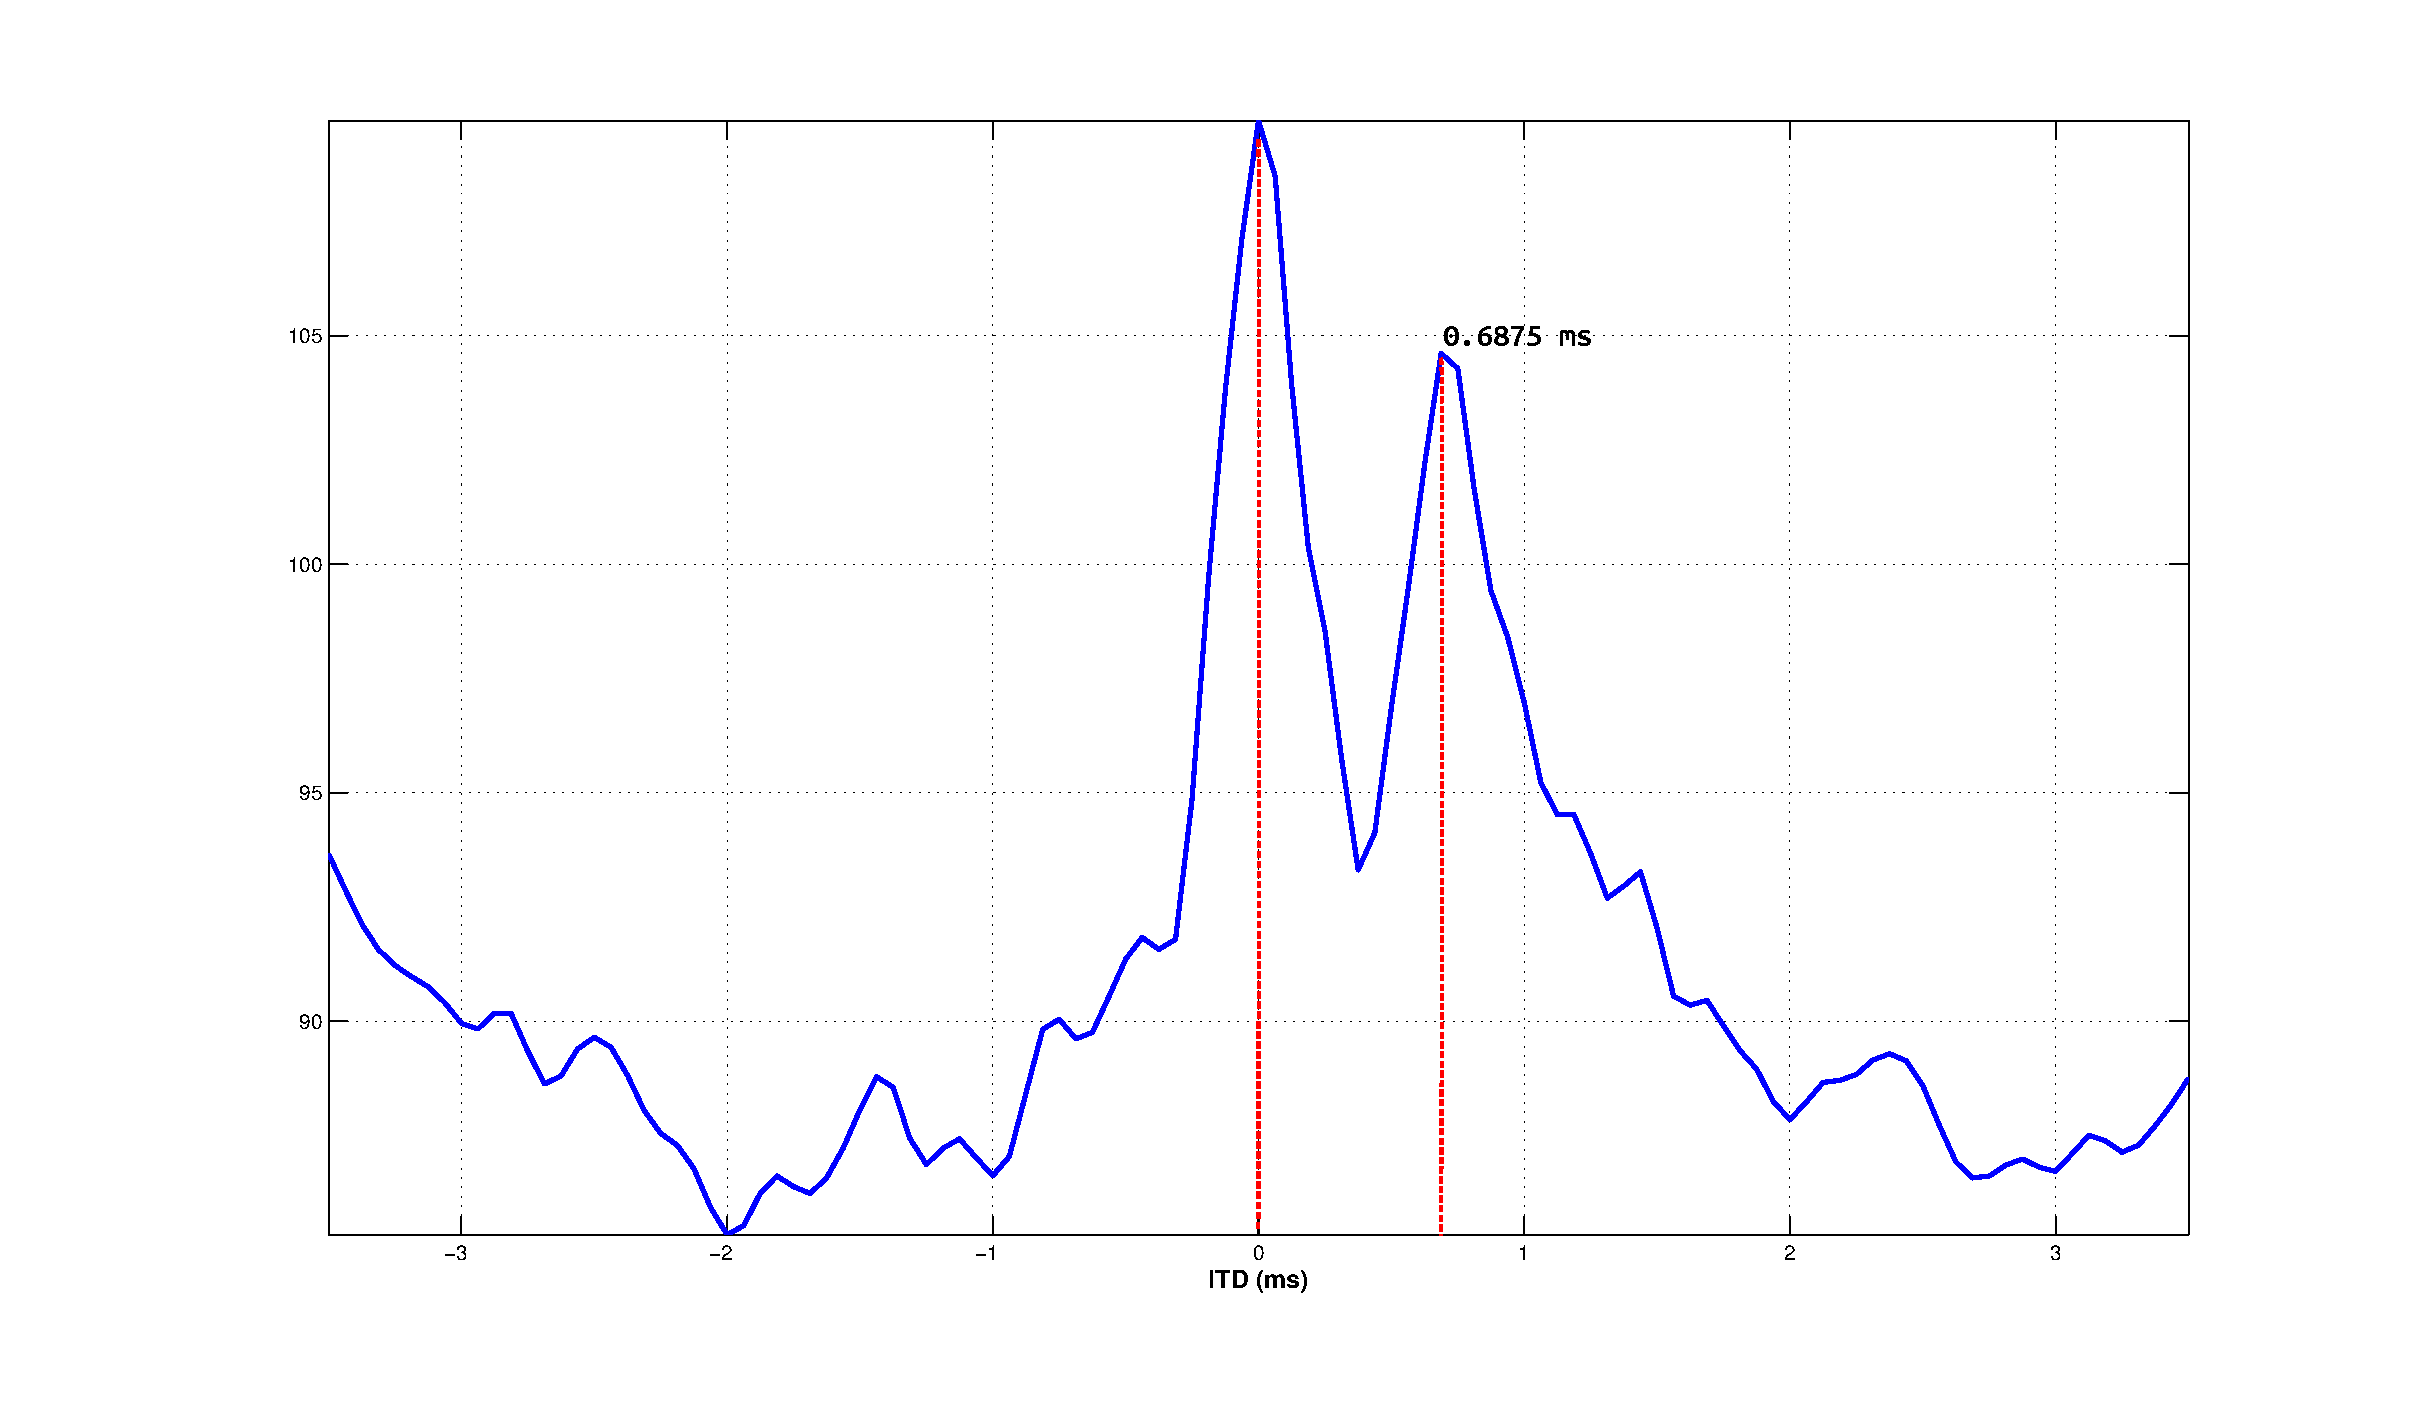
\includegraphics[width=5.5in]{pict/azimuth.eps}
%	\begin{minipage}[b]{14pc}
    \caption{\label{pict:azimuth}The sum of cross-correlation between mixtured signal at left ear and right ear}
%	\end{minipage}
\end{figure} 

\subsection{Binary Mask Estimation}
Binary mask is estimated at each time-frequency unit. The binary mask value is 1 if the value of PDE with $RS > 0.5$ in figure \ref{pict:pde} (a) is greater than PDE with $RS \leq 0.5$ in figure \ref{pict:pde} (b) and will be 0 if the value of PDE with $RS > 0.5$ in figure \ref{pict:pde} (a) less than or equal to the PDE $RS \leq 0.5$ in figure \ref{pict:pde} (b). The value of each PDE obtained from ITD and ILD masker signal in each unit time-frequency of the mixtured signal. In figure \ref{pict:pde} is a graph of the PDE of a target at azimuth $0^o$ and a masker at azimuth $30^o$ with the center frequency of 500 Hz and SIR 10 dB. ITD and ILD masker obtained at center frequency of 500 Hz, calculated the value of its binary mask based on the probability density estimation in figure \ref{pict:pde}. Figure \ref{pict:spect_est_sig} shown spectrogram of estimated target signal compare to clean target signal and mixtured target signal.

\begin{figure}[h]
    \centering
    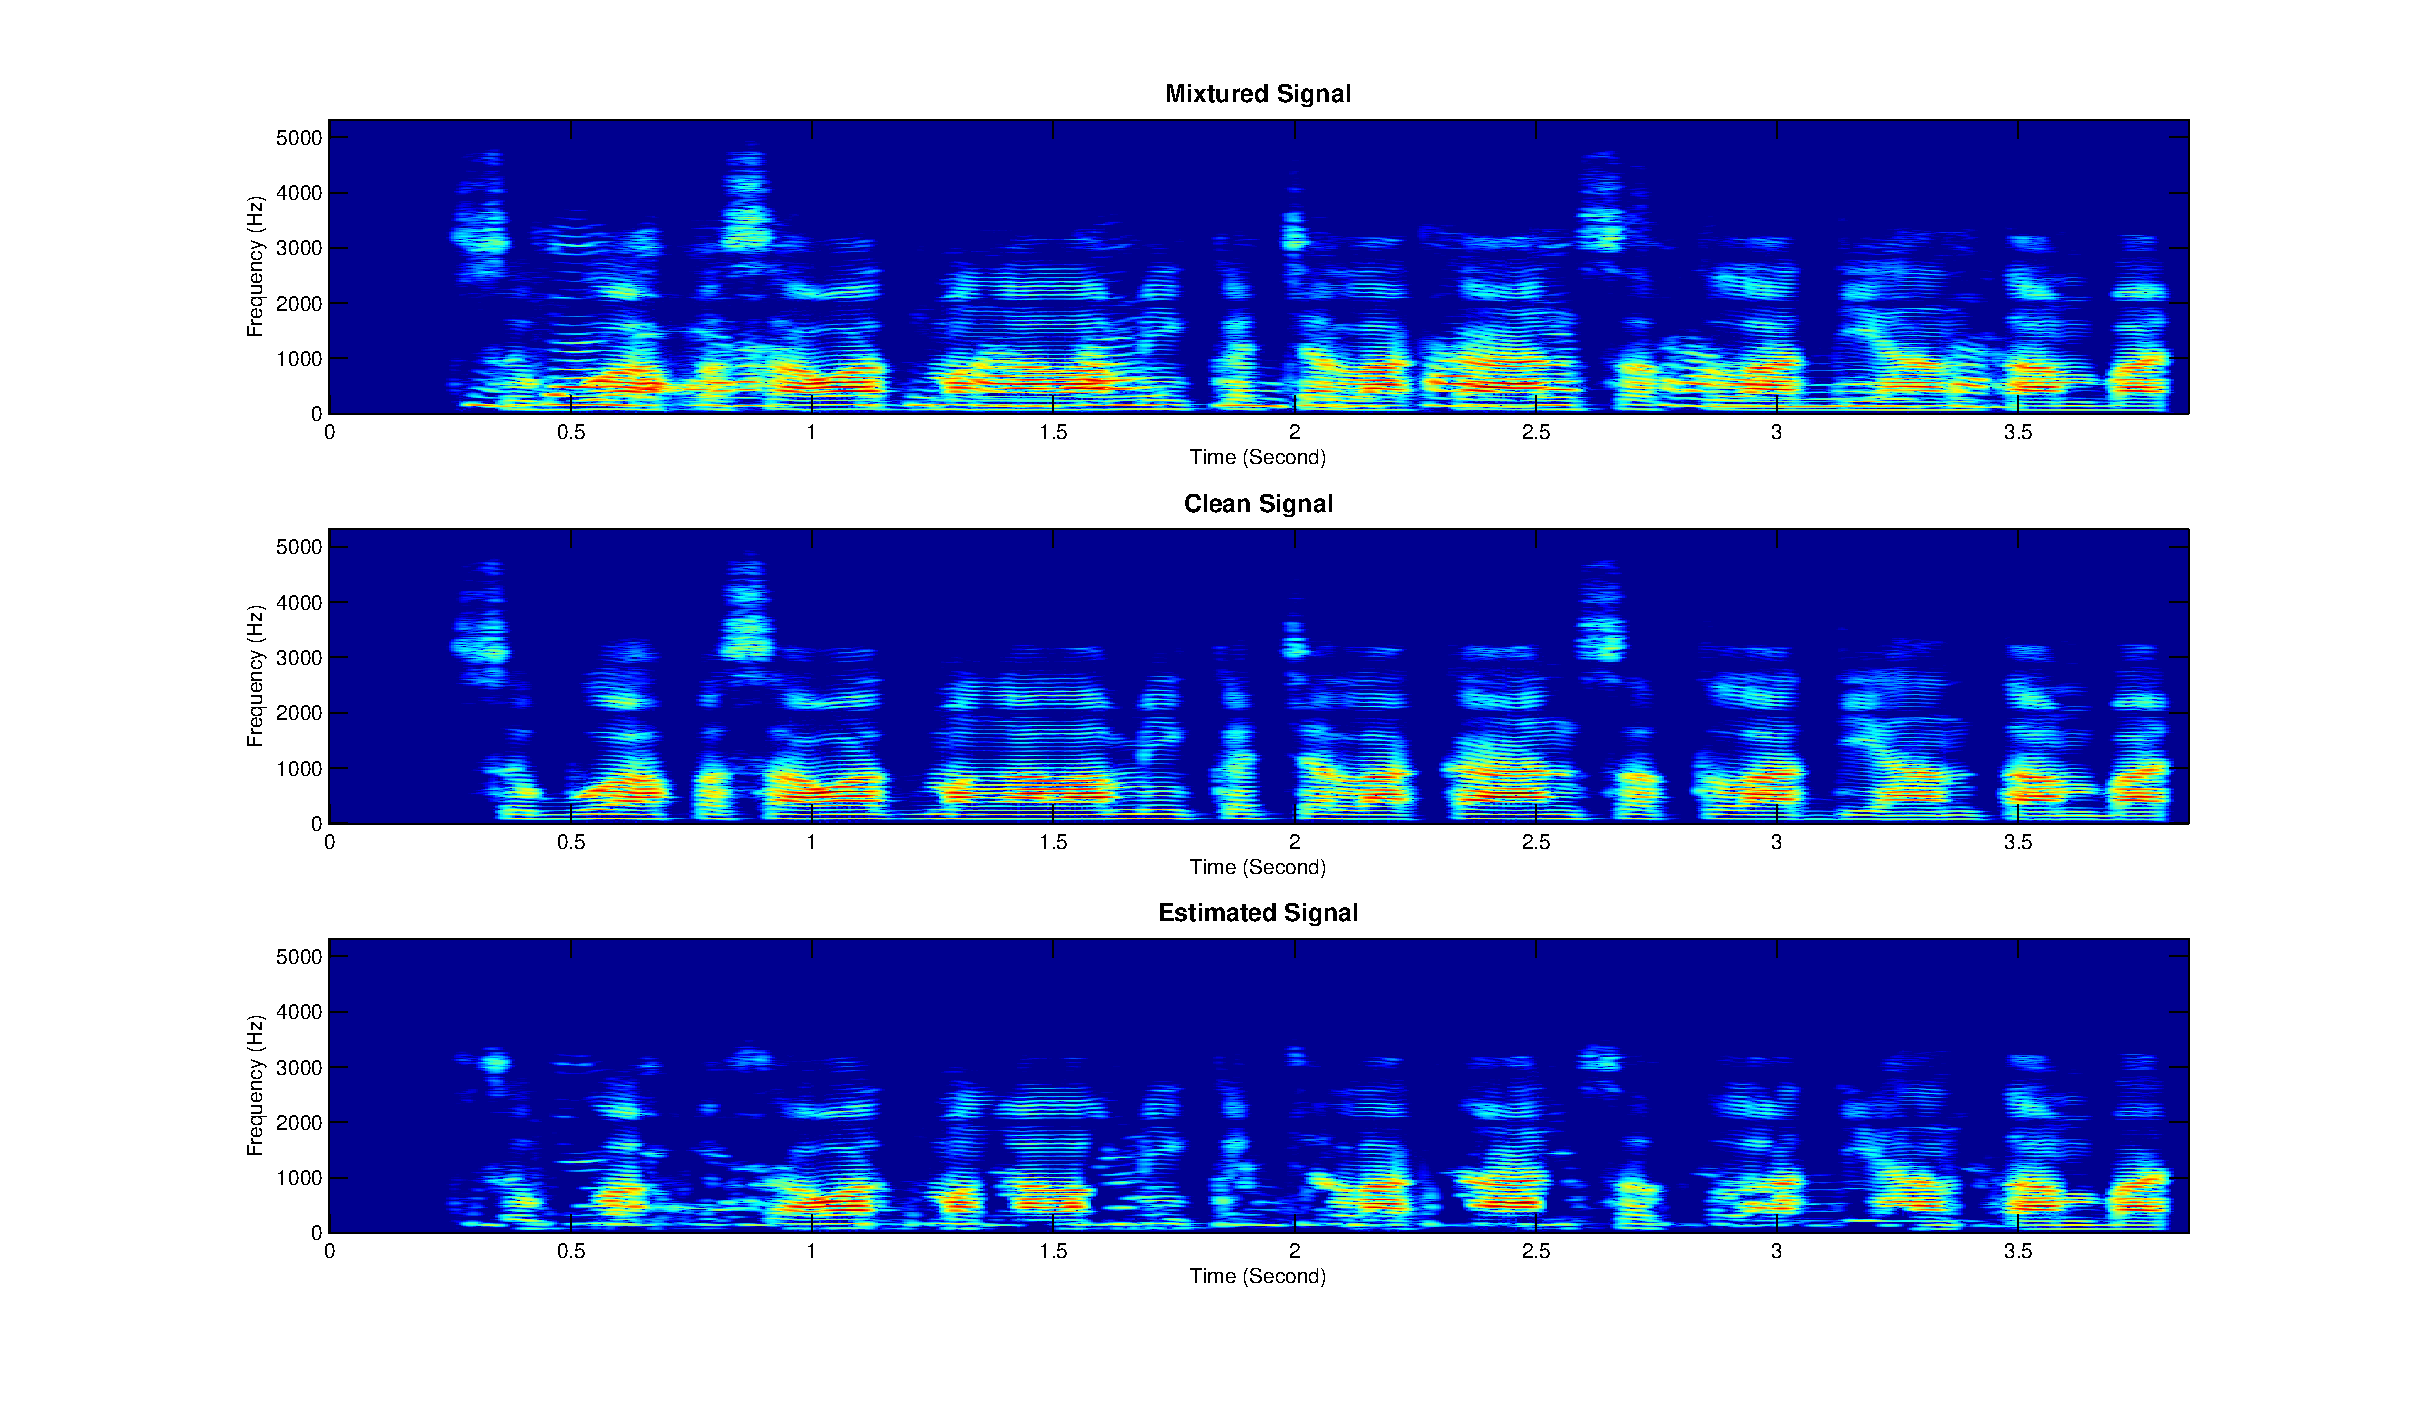
\includegraphics[width=7in]{pict/spectrogram_results.eps}
%	\begin{minipage}[b]{14pc}
    \caption{\label{pict:spect_est_sig}Spectrogram of (a) mixtured signal, (b) clean target signal and (c) estimated target signal}
%	\end{minipage}
\end{figure} 

\section{Evaluation}
Evaluation method that used is percent correct word for subjective evaluation that shown in figure \ref{pict:eval_pcw} and SNR for objective evaluation that shown in figure \ref{pict:eval_snr}.

\begin{figure}[h]
    \centering
    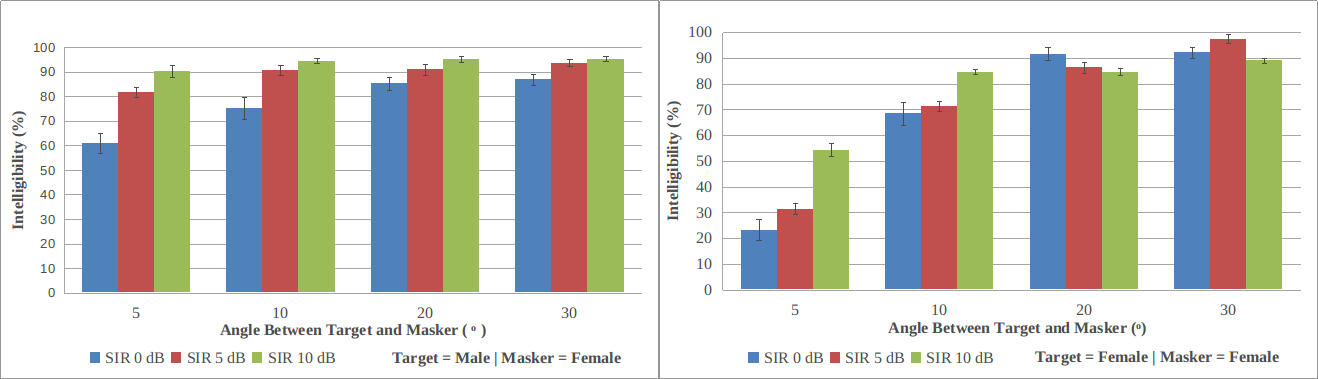
\includegraphics[width=5.5in]{pict/evaluation_pcw.png}
%	\begin{minipage}[b]{14pc}
    \caption{\label{pict:eval_pcw}Evaluation using percent correct words with target male speaker and masker female speaker}
%	\end{minipage}
\end{figure} 

\begin{figure}[h]
    \centering
    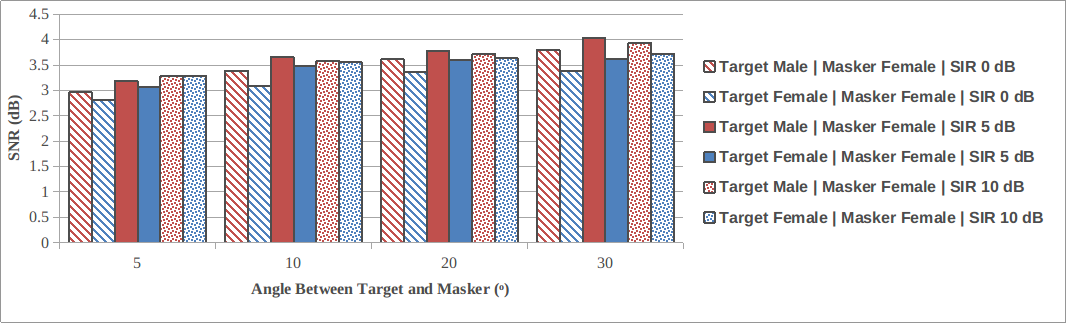
\includegraphics[width=5.5in]{pict/evaluation_snr.png}
%	\begin{minipage}[b]{14pc}
    \caption{\label{pict:eval_snr}Evaluation using SNR with variation of speaker and angle separator between target and masker}
%	\end{minipage}
\end{figure} 

\section{Result and Discussion}
Based on the results of subjective evaluation in figure \ref{pict:eval_pcw}, the larger angle and SIR between target and masker signal then speech intelligibility of separation result is increase. For a different speaker between the target and masker signal, has a higher speech intelligibility than the same speaker of target and masker signal. So as for the results of an objective evaluation in figure \ref{pict:eval_snr}, the larger angle and SIR between target and masker signal then SNR of separation result is increases. For a different speaker between the target and masker signal, has a higher SNR than the same speaker of target and masker signal.


In figure \ref{pict:eval_pcw}, the increase of speech intelligibility with 0 dB SIR looks significantly by $60\%$ in $5^o$, $75\%$ in $10^o$, $85\%$ in $20^o$ and $86\%$ in $30^o$. Similarly to 5 dB SIR. Meanwhile for 10 dB SIR, speech intelligibility is not very significant increased, which is $90.1\%$ in $5^o$, $94.4\%$ in $10^o$, $95.3\%$ in $20^o$ and $95.4\%$ in $30^o$.

\section{Conclusion}
The sound quality of separation results for the same speaker between the target and masker signal smaller, that is $72.86\%$ correct words and 3.38 dB SNR, than different speaker that is $86.74\%$ correct words and 3.5 dB SNR.

\section*{References}
\begin{thebibliography}{9}
	\bibitem{kates2008}
		Kates J M 2008 {\it Digital Hearing Aids} (San Diego: Plural Publishing)
	\bibitem{marin2012}
	Marin J 2012 Robust Noise Reduction Strategies For Binaural Hearing Aids {\it PhD thesis} (Georgia Institute of Technology)
	\bibitem{cherry1957}
		Cherry C 1957 {\it On human communication; a review, a survey, and a criticism} (Cambridge: Technology Press of Massachusetts Institute of Technology)
	\bibitem{hawley2004}
		Hawley M L, Litovsky R Y, and Culling J F 2004 The benefit of binaural hearing in a cocktail party: effect of location and type of interferer {\it J. Acoust. Soc. Am.} {\bf 115} 833.
	\bibitem{roman2002}
		Roman N, Wang D, Brown G J 2002 Speech segregation based on sound localization {\it J. Acoust. Soc. Am.} {\bf 114} 2236
	\bibitem{meddis1986}
		Meddis R 1986 Simulation of mechanical to neural transduction in the auditory receptor {\it J. Acoust. Soc. Am.} {\bf 79} 702
	\bibitem{jeffress1948}
		Jeffress L A 1948 A place theory of sound localization {\it Journal of comparative and physiological psychology} {\bf 41}(1) 35
\end{thebibliography}
\end{document}


